\documentclass[11pt]{article}
\usepackage{graphicx}
\usepackage{array}
\usepackage{xcolor}
\usepackage[a4paper,total={8in,10in}]{geometry}
\usepackage{mdframed}
\usepackage{geometry}
\usepackage{hyperref}
\begin{document}
\begin{mdframed}[backgroundcolor=black]
~
\begin{center}
\begin{Huge}
\color{white}{\fontfamily{pbk}\selectfont Chetan}\color{gray}{\fontfamily{pbk}\selectfont\textbf{Chawla}}
\end{Huge}
\end{center}
\begin{center}
\begin{large}
\color{white}\emph{I am not a perfectionist , but I do have the will it takes}
\end{large}
\end{center}
\end{mdframed}
\begin{minipage}{0.25\linewidth}
\begin{center}
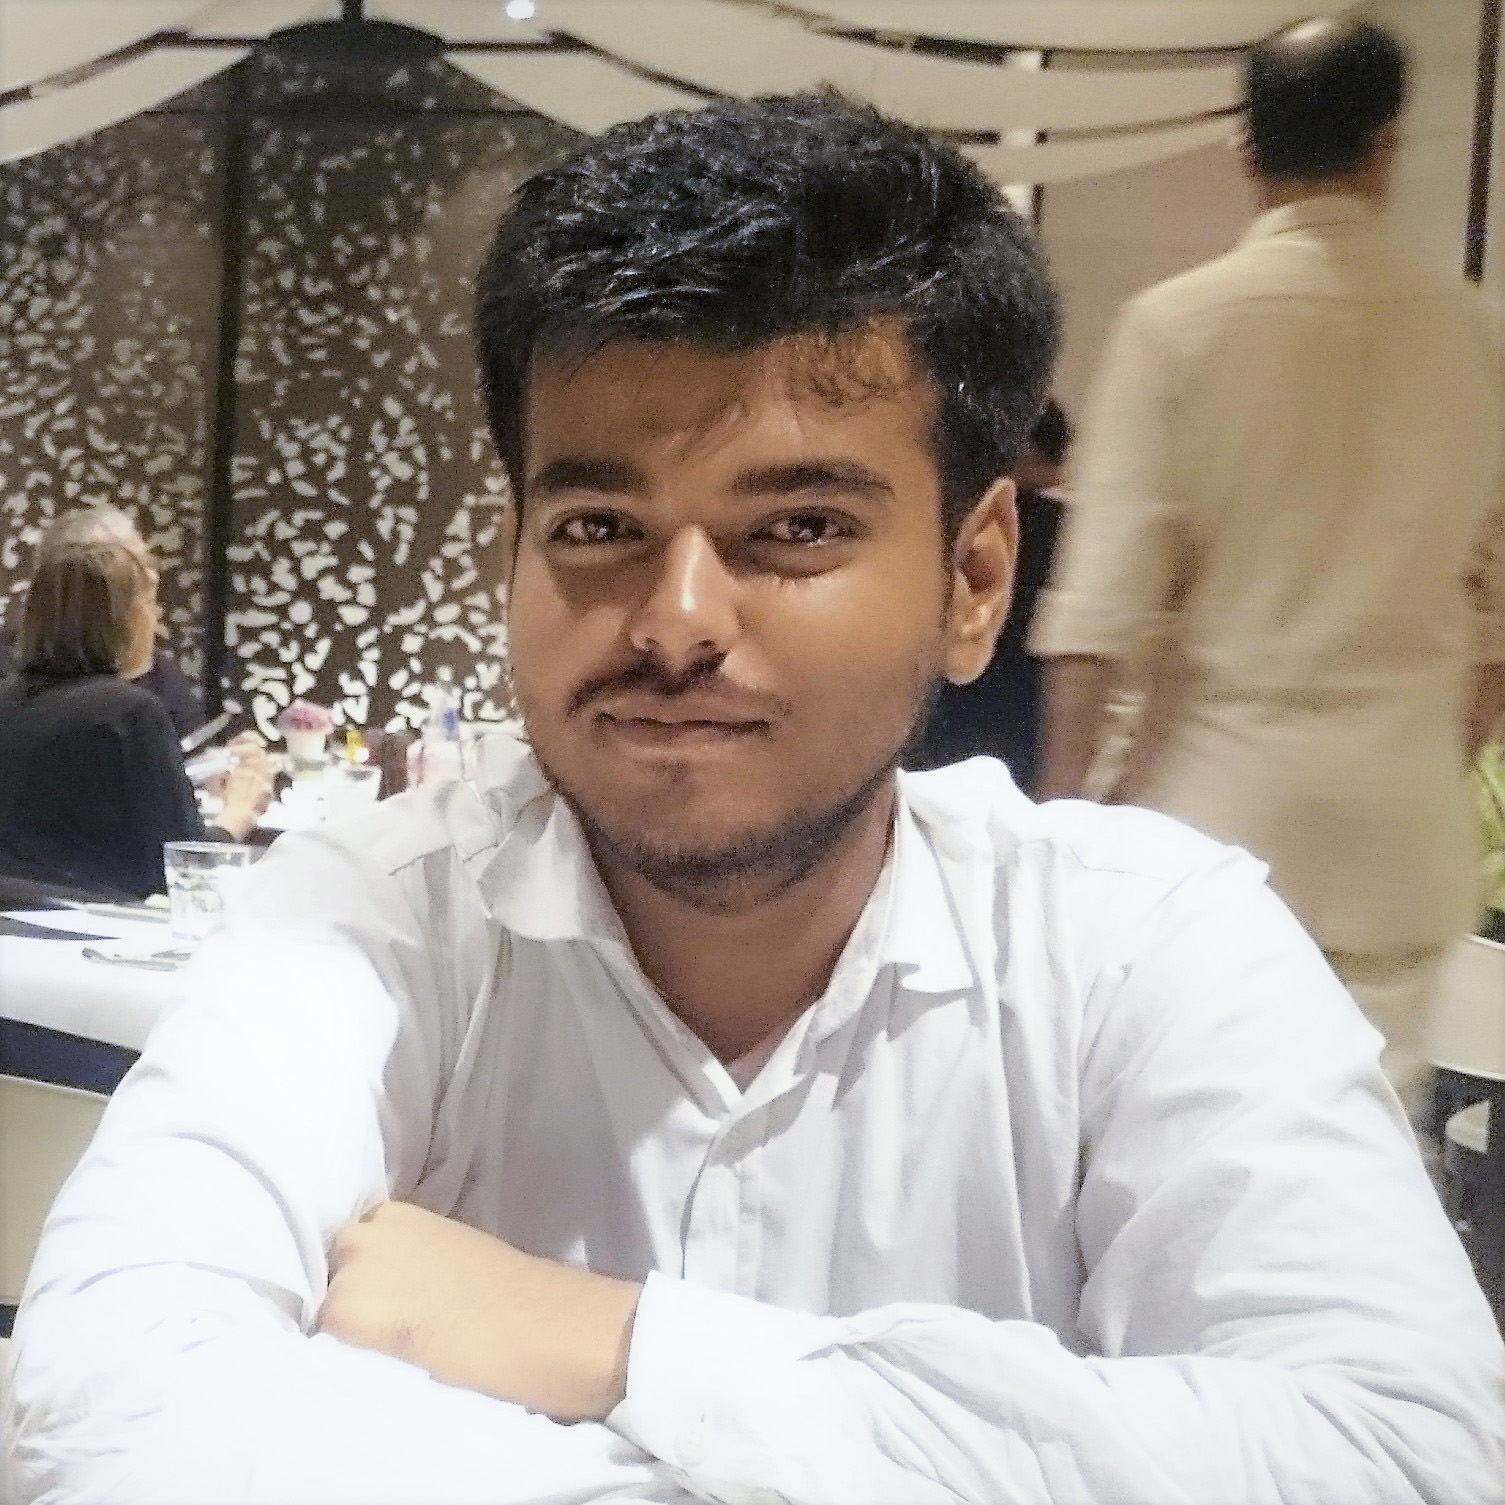
\includegraphics[scale=0.085]{picture}
\end{center}
\begin{flushright}
	\section{\color{green}Per\color{purple}s\color{black}onal D\color{purple}e\color{black}tai\color{purple}l\color{black}s}
    C-4  
    Tagore Garden Extn.\\
    New Delhi\\
    110027\\
    ~
    \textbf{Contact}-\\
    +91 9013307073\\
    ~
    \textbf{E-mail-}\\
    \href{mailto:chchawla@yahoo.co.in}{chchawla@yahoo.co.in}
    \textbf{LinkedIn-}\\
    \href{http://bit.ly/2ioNlFC}{http://bit.ly/2ioNlFC}
\end{flushright}

\end{minipage}
\begin{minipage}{0.75\linewidth}

\section{\color{red}Car\color{purple}e\color{black}er Obje\color{purple}ct\color{black}ive}
Having happiness and being content in what you do is the most important thing for me. I have a passion for astronomy and astrophysics, thus I would be \textbf{working towards joining ISRO} and serving humanity.
\section{\color{yellow}Edu\color{black}cational Qualifications}
\begin{center}
\begin{tabular}{ |m{4cm}| m{4cm}| m{2cm}| m{3cm}| }
\hline
&&&\\
\begin{center}
\textbf{{ Course/Examination }}
\end{center}&\begin{center}\textbf{ Institute/University }\end{center}&\begin{center}\textbf{ Year of passing }\end{center}&\begin{center}\textbf{ Performance }\end{center}\\
\hline
&&&\\
\begin{center}
B.Tech, Electronics and Communication Engineering
\end{center}& \begin{center}
Bharati Vidyapeeth's College Of Engineering
\end{center}&\begin{center}
2019
\end{center}& \begin{center}
82.3494 (C) (up to third semester)
\end{center}\\
\hline
\begin{center}
AISSCE (SCIENCE-PCMB)\\
XIIth
\end{center}&
\begin{center}
(CBSE) Kendriya Vidyalaya Tagore Garden, New Delhi
\end{center}&
\begin{center}
2015
\end{center}&
\begin{center}
95.00 percent(agg)
\end{center}\\
\hline
\begin{center}
AISSE\\
Xth
\end{center}&
\begin{center}
(CBSE) Kendriya Vidyalaya Tagore Garden, New Delhi
\end{center}&
\begin{center}
2013
\end{center}&
\begin{center}
93.10 percent
\end{center}\\
\hline
\end{tabular}
\end{center}
\section{\color{orange}Pro\color{black}jects}
\subsection{Co\color{purple}m\color{black}pl\color{purple}e\color{black}ted}
\begin{enumerate}
\item Swarm robotics using Serial communication between two Firebird V s (XBees 2.4C)
\item Interfacing Firebird V, eYRC Labs, IIT Bombay(ATMEGA2560)
\item Note Identification System using Audio Processing-Python Based
\item IR based invisible piano( ATMEGA16 platform)
\item Propeller Clock  (ATMEGA8)
\item IoT based Door lock system (TI- CC3200)
\item Bluetooth Module Controlled Wireless Differential Drive Bot (HC05)
\end{enumerate}
\end{minipage}

\begin{minipage}{0.20\linewidth}
~\\
\end{minipage}
\begin{minipage}{0.80\linewidth}
\subsection{Completed-Continued}
\begin{enumerate}
\item DTMF controlled home automation (Arduino and ATMEGA16)
\item Line follower robot (based on L293D and 7805 only)
\item Hydraulics Arm
\item Motor controlled gear steered bot using DPDT
\item Calculator application for android
\end{enumerate}

\subsection{Currently Working On}
\begin{enumerate}
\item Semi-Automated Car –Lane, pedestrian and car avoidance system (Raspberry Pi and\\ DIP). Celestini by Princeton University.
\item HexaPod: Line following/ HC05 interfacing/ Path tracer/ Obstacle detector, avoider\\ and carrier.
\item X-Copter (Quadcopter)  using KK2 pilot board.
\item Water purification system using refrigerators
\item Tesla Coils
\item Visible Light Communication(VLC)- Advanced version of LiFi
\end{enumerate}
\section{\color{pink}Tra\color{black}ining and Internships}
\begin{itemize}
\item Introduction to Java- Workshop series by GDG-BVP [January-March 2017]
\item 14 hr. workshop series by Texas Instruments Ltd. On Embedded Systems and\\ Internet of Things[October 2016]
\item \textbf{Training on Embedded Systems} (Cyborg Labs) [June-August 2016]
\item \textbf{Android development for beginners} (Udacity) [February-April 2016]
\item \textbf{Workshops on Arduino based controlling}/Robotic workshops(8) by RAS,\\ BVPIEEE [October 2016-Present]
\item Workshops on Competitive Coding by Google Developers Group,BVCOE
\item Workshop on Embedded Systems by CETPA Info-tech Ltd. (BVCOE)
\end{itemize}

\section{\color{blue}Res\color{black}earch and Publications}
\begin{enumerate}
\item None as of now
\end{enumerate}

\section{\color{cyan}Tec\color{black}hnical Skills}
\subsection{Programming Languages}
\begin{itemize}
\item C
\item XML for android development
\item Python Basics
\item Embedded C
\end{itemize}
\end{minipage}
\begin{minipage}{0.20\linewidth}
~\\
\end{minipage}
\begin{minipage}{0.80\linewidth}
\subsection{Operating Systems}
\begin{itemize}
\item Windows XP/7/8/10
\item Android
\end{itemize}
\subsection{Software and Platforms worked upon}
\begin{itemize}
\item Microsoft Office
\item Arduino IDE
\item Android Studio
\item Proteus
\item Energia
\item TeraTerm
\item XCTU
\item Sinaprog
\item Audacity
\item KK multicopter flash tool
\item LaTeX
\end{itemize}
\subsection{Others}
\begin{itemize}
\item Orcad Capture
\item AVR Studio
\item Blender GUI
\item Audio Processing
\end{itemize}
\subsection{Development Boards/Modules}
\begin{itemize}
\item ATMEGA16
\item Arduino Mega(ATMega 2560) and Uno(ATMega328)
\item MSP430(LaunchPad)
\item CC3200(built in accelerometer)
\item HC05
\end{itemize}

\end{minipage}
\end{document}